\level{2}{Chuck}
	\begin{figure}[H]\centering
        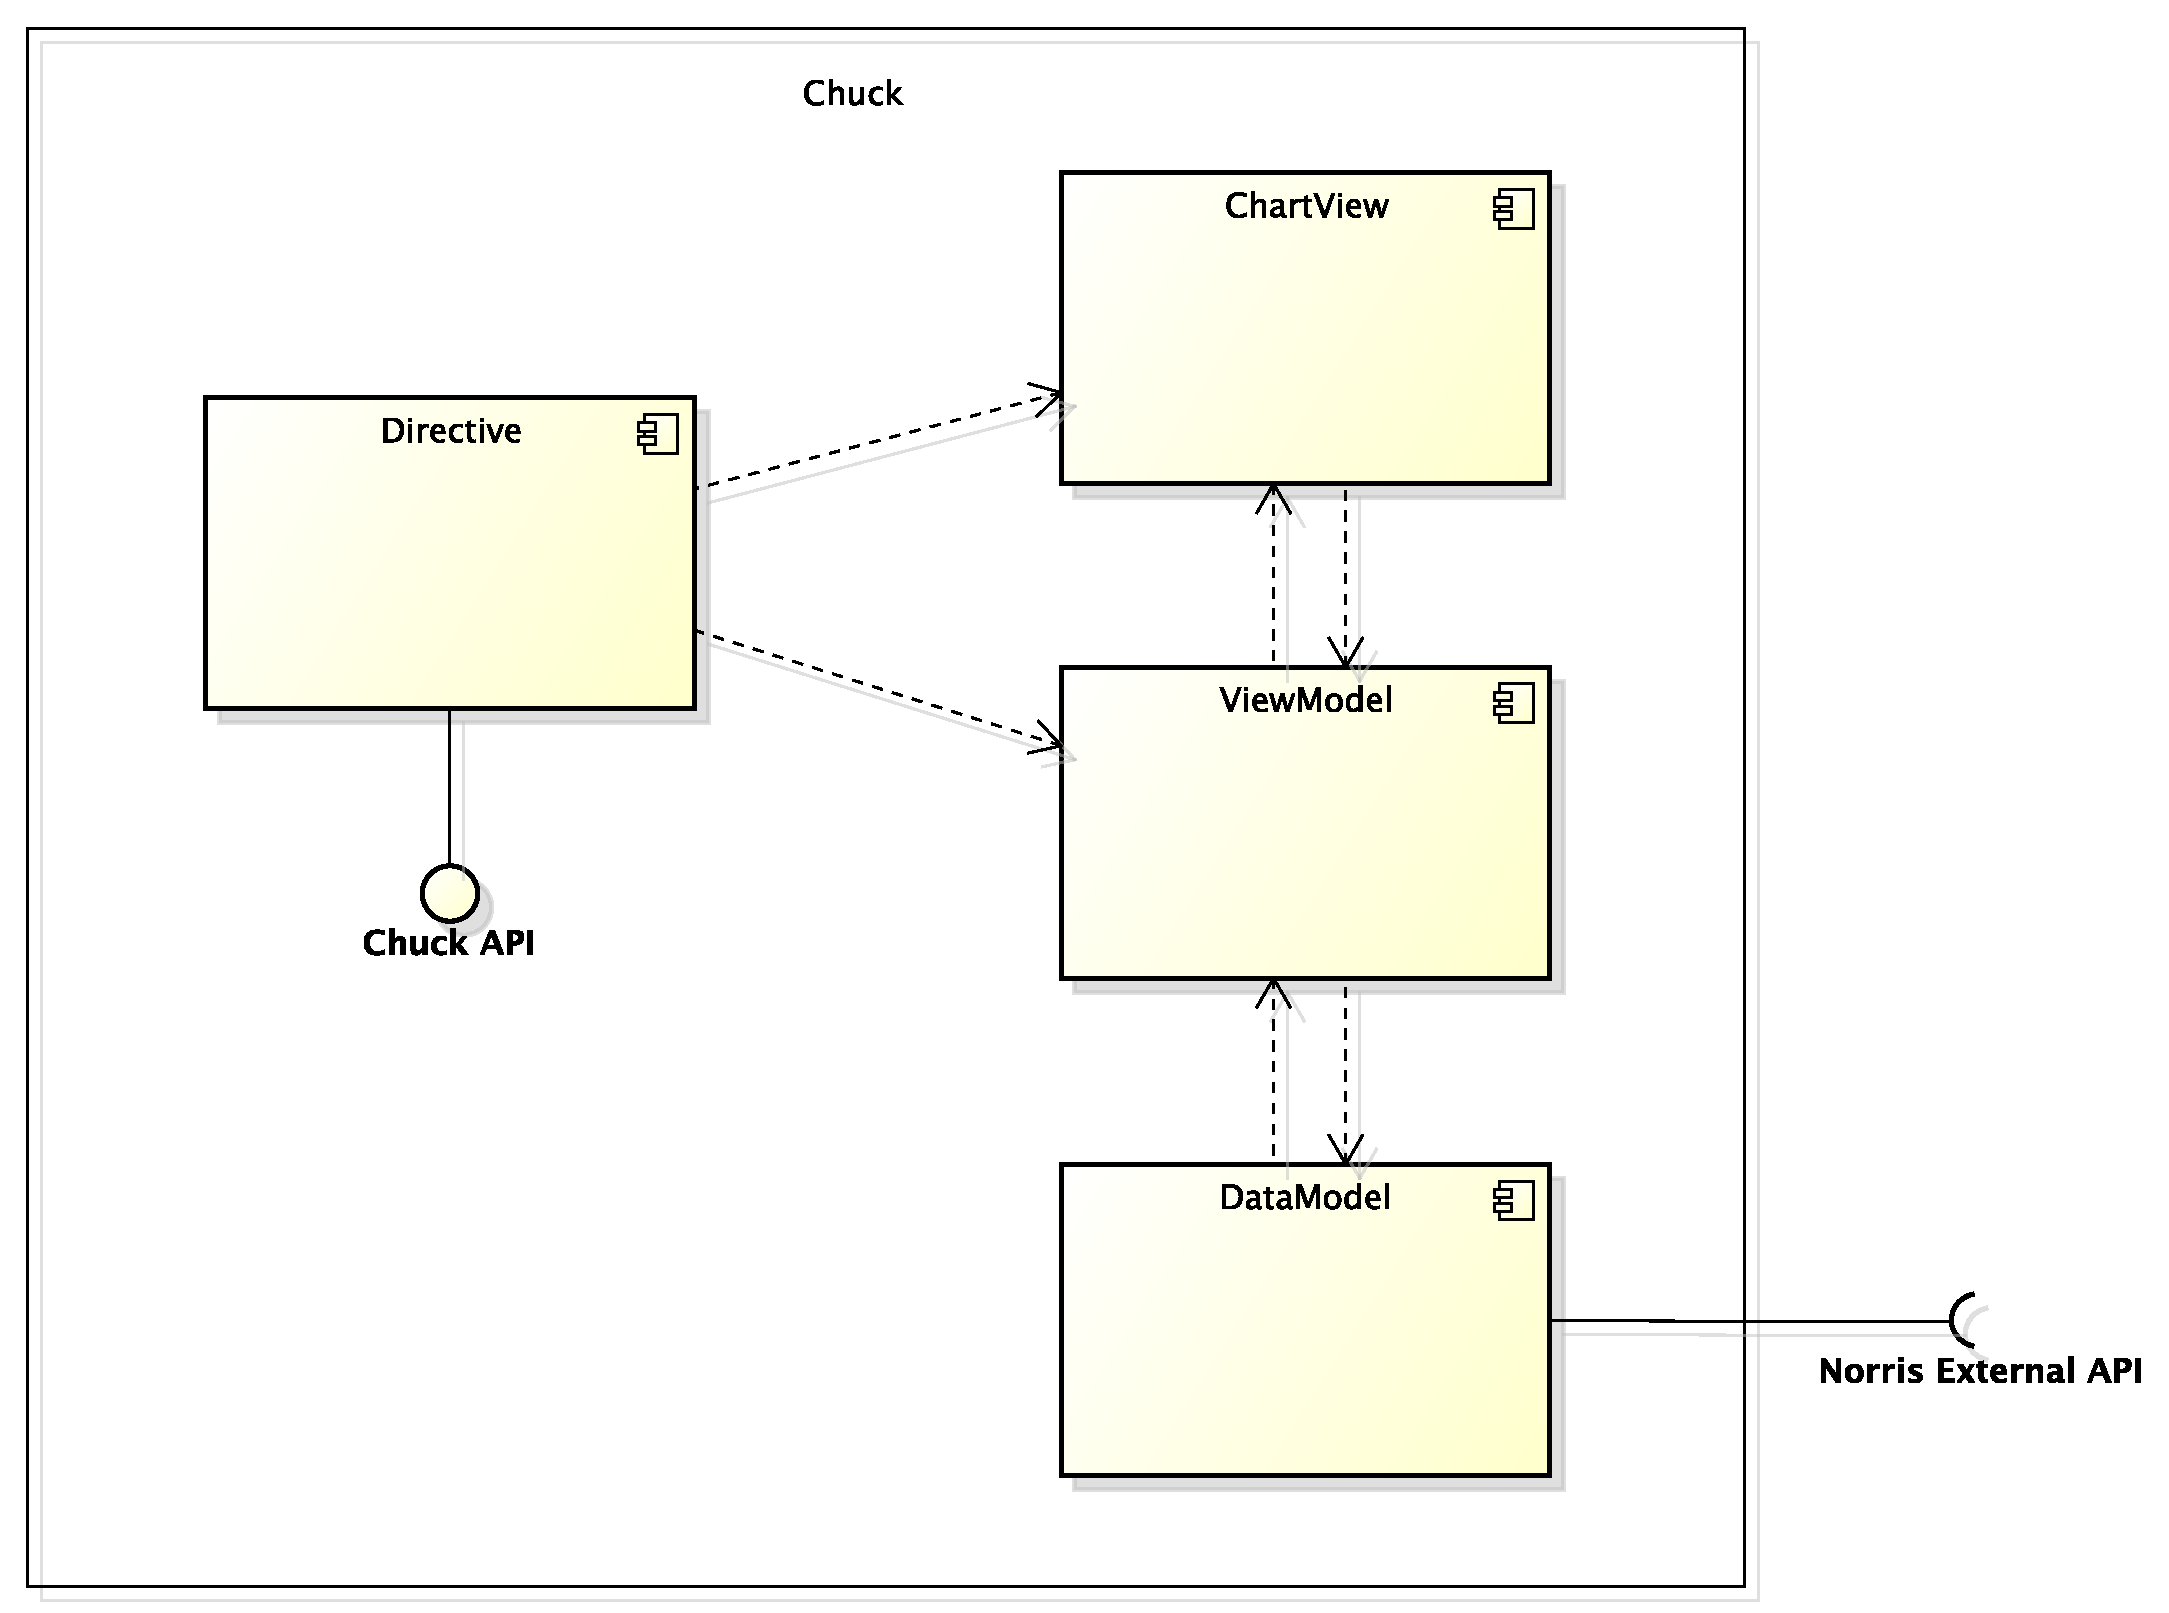
\includegraphics[width=\textwidth]{SpecificaTecnica/Pics/ComponentiChuck}
        \caption{Diagramma delle componenti di Chuck}
    \end{figure}
	\level{3}{Descrizione delle componenti di Chuck}
    	\level{4}{Model}
			La componente Model è un modello che astrae i grafici visualizzati nella pagina web. Si divide a sua volta in due sottocomponenti:
			\begin{itemize}
				\item NorrisChart: contiene i dati riguardanti i grafici, assieme alle relative impostazioni. In particolare sono presenti i modelli di tutte le tipologie di chart implementati da Norris, ovvero Bar Chart, Line Chart, Map Chart e Table. Per ciascuna tipologia di grafico sono forniti i metodi per inserire i dati e configurare alcune impostazioni. Fornisce inoltre dei metodi per ottenere i valori di queste ultime, in modo da poterle riutilizzare per un altro grafico. Infine, per ogni grafico sono disponibili le stesse modalità di aggiornamento fornite da Norris.
				\item Services: si occupa della comunicazione con Norris attraverso l'utilizzo delle API esterne. In particolare gestisce le richieste dei grafici che lo sviluppatore client vuole inserire nel proprio sito e la ricezione degli aggiornamenti dei grafici stessi. Gestisce inoltre l'autenticazione presso l'istanza di Norris contenente tali grafici, fornendo allo sviluppatore le funzioni di login e logout.
			\end{itemize}

		\level{4}{Directive}
			La componente Directive fornisce le principali API di Chuck allo sviluppatore client. Le funzionalità offerte sono le seguenti:
			\begin{itemize}
				\item inserire nuovi grafici in un sito web;
				\item scegliere i grafici da inserire;
				\item scegliere il tag HTML in cui inserire un grafico;
				\item modificare alcune impostazioni dei grafici.
			\end{itemize}
			Questa componente comunica le sccelte dell'utente al ViewModel e alla View.
    		
		\level{4}{View}
			La componente View ha il compito di visualizzare i grafici all'interno della pagina web. I grafici possono essere del tipo Bar Chart, Line Chart, Map Chart e Table. Quando un grafico viene aggiornato, questa componente si occupa di aggiornare anche la sua visualizzazione nella pagina web. Un altro compito della View consiste nell'accogliere gli input inerenti il filtraggio dei dati di un determinato chart e inviarli al ViewModel.
			
		\level{4}{View Model}
			La componente ViewModel fa da tramite tra la View e il Model. Si occupa di richiamare le funzionalità delle librerie grafiche che permettono alla View di visualizzare i grafici. Inoltre ha lo scopo di ricevere gli input provenienti dalla View ed effettuarne la gestione. L'input consiste in un sottoinsieme di dataset scelti dall'utente che sta visualizzando la pagina web. Il ViewModel deve far sì che vengano visualizzati solo questi dataset, in modo da permettere all'utente di applicare un filtro sulle serie.
			    
	\level{3}{Descrizione delle interazioni tra le componenti}
		\level{4}{Model - ViewModel}
			Quando avviene una modifica nel Model, una notifica avvisa il ViewModel dell'avvenuto cambiamento. In particolare quando arriva l'aggiormento di un grafico già presente, dopo aver aggiornato i dati del grafico il Model manda una notifica al ViewModel.

		\level{4}{ViewModel - Model}
			Quando il ViewModel deve aggiornare la visualizzazione del grafico, esso effettua una query sul Model per ottenere le nuove informazioni relative al grafico da aggiornare. Ciò avviene dopo che il ViewModel è stato notificato riguardo un cambiamento avvenuto nel Model. 
			
		\level{4}{View - ViewModel}
			Quando la View riceve un input dall'utente, una notifica avvisa il ViewModel in modo che intraprenda l'azione per gestirla. In particolare la View notifica il ViewModel quando l'utente seleziona i dataset che vuole visualizzare. La View invia al ViewModel anche le informazioni relative ai dataset selezionati, in modo che quets'ultimo possa effettuare le operazioni di filtraggio dei dati.
			
		\level{4}{ViewModel - View}
			Il ViewModel si occupa di aggiornare la View quando i dati del Model vengono modificati. In particolare ciò avviene dopo l'inserimento di un nuovo grafico o dopo un aggiornamento. Inoltre il ViewModel si occupa di modificare la View in seguito ad una richiesta di filtraggio dei dati.
				
		\level{4}{Directive - ViewModel}
			La Directive demanda l'implementazione delle funzionalità fornite dalle API di Chuck ai metodi del ViewModel. Si occupa dunque di richiamare i metodi del ViewModel necessari, passando loro i parametri corretti.
			
		\level{4}{Directive - View}
			La Directive si occupa di selezionare la View corrispondente al tipo di grafico che si vuole inserire nella pagina web.
	\level{3}{Design pattern utilizzati}
		Riportiamo di seguito i pattern architetturali utilizzati nella progettazione delle componenti di Chuck.
		\level{4}{Model View ViewModel}
			Model-View-ViewModel (MVVM) è un pattern architetturale utilizzato per separare il codice in blocchi di funzionalità ben distinte.\\
			Per la descrizione del pattern e dei vantaggi derivanti dalla sua applicazione si rimanda all'appendice \nameref{app:???}.
			\level{5}{Contesto di utilizzo}
				L'MVVM viene utilizzato per dividere le classi della libreria Chuck in tre grandi componenti:
				\begin{itemize}
					\item View;
					\item Model;
					\item ViewModel;
				\end{itemize}
	
